\documentclass[11pt,a4paper]{article}

% Pacotes essenciais
\usepackage[utf8]{inputenc}
\usepackage[T1]{fontenc}
\usepackage[portuguese]{babel}

% --- TIPOGRAFIA (do modelo) ---
\usepackage{mathptmx}
\usepackage{microtype}
% ------------------------------

\usepackage{geometry}
\geometry{a4paper, margin=2.5cm}
\usepackage{graphicx}
\usepackage{hyperref}
\usepackage{float}
\usepackage{listings}
\usepackage{xcolor}
\usepackage{titlesec}
\usepackage{caption}
% Cada título (section) começa em página nova
\AddToHook{cmd/section/before}{\clearpage}
\usepackage{tikz}
\usetikzlibrary{shapes.geometric, arrows, positioning, fit, calc}

\renewcommand{\arraystretch}{1.15}

\addto\captionsportuguese{
  \renewcommand{\lstlistingname}{Código}
  \renewcommand{\lstlistlistingname}{Índice de Códigos}
}

\definecolor{codegray}{rgb}{0.5,0.5,0.5}
\definecolor{backcolour}{rgb}{0.95,0.95,0.92}
\definecolor{upca}{HTML}{29ABE2}

\lstdefinestyle{mystyle}{
    backgroundcolor=\color{backcolour},
    commentstyle=\color{codegray},
    keywordstyle=\color{blue},
    numberstyle=\tiny\color{codegray},
    stringstyle=\color{orange},
    basicstyle=\ttfamily\footnotesize,
    breakatwhitespace=false,
    breaklines=true,
    captionpos=b,
    keepspaces=true,
    numbers=left,
    numbersep=5pt,
    showspaces=false,
    showstringspaces=false,
    showtabs=false,
    tabsize=2,
    literate={á}{{\'a}}1 {é}{{\'e}}1 {í}{{\'i}}1 {ó}{{\'o}}1 {ú}{{\'u}}1
             {Á}{{\'A}}1 {É}{{\'E}}1 {Í}{{\'I}}1 {Ó}{{\'O}}1 {Ú}{{\'U}}1
             {à}{{\`a}}1 {è}{{\`e}}1 {ì}{{\`i}}1 {ò}{{\`o}}1 {ù}{{\`u}}1
             {À}{{\`A}}1 {È}{{\`E}}1 {Ì}{{\`I}}1 {Ò}{{\`O}}1 {Ù}{{\`U}}1
             {ã}{{\~a}}1 {õ}{{\~o}}1 {Ã}{{\~A}}1 {Õ}{{\~O}}1
             {â}{{\^a}}1 {ê}{{\^e}}1 {î}{{\^i}}1 {ô}{{\^o}}1 {û}{{\^u}}1
             {ç}{{\c{c}}}1 {Ç}{{\c{C}}}1 {º}{{\textsuperscript{o}}}1 {ª}{{\textsuperscript{a}}}1
}
\lstset{style=mystyle}

\begin{document}

% Capa (estilo do modelo, conteúdo ISI)
\begin{titlepage}
    \centering
    \vspace*{0.4cm}
    % Logo UPCA (PNG com faixa branca a direita: compensacao para centragem otica)
    \hspace*{0.035\textwidth}
\includegraphics[width=0.3\textwidth]{imagens/logo_upca.png}

    \vspace{0.7cm}
    {\scshape\large Instituto Politécnico do Cávado e do Ave\par}
    \vspace{0.15cm}
    {\scshape\LARGE Escola Superior de Tecnologia\par}

    \vspace{0.5cm}
    {\color{upca}\rule{\textwidth}{1.2pt}}\par

    \vspace{0.5cm}
    {\large Licenciatura em Engenharia de Sistemas Informáticos\par}
    \vspace{0.15cm}
    {\large Unidade Curricular de Integração de Sistemas de Informação\par}
    \vspace{0.15cm}
    {\large 2026/27\par}

    \vfill

    {\huge\bfseries Trabalho Prático I\par}
    \vspace{0.7cm}
    {\color{upca}\rule{0.55\textwidth}{0.9pt}}\par
    \vspace{0.7cm}
    {\LARGE ISI Store --- Loja E-commerce\par}
    \vspace{0.25cm}
    {\Large Processo \textit{Extract, Transform and Load} (ETL)\par}

    \vfill

    {\large
    \begin{tabular}{r@{\quad}l}
      \textbf{Autor:} & Tiago Fontes \\
      \textbf{Número:} & 33222 \\
      \textbf{Email:} & \url{a33222@alunos.ipca.pt} \\
      \textbf{Repositório Git:} & \url{https://github.com/Fontes9/Trabalho-Pr-tico-I---ISI} \\
    \end{tabular}\par}

    \vspace{1.2cm}
    {\large \today\par}
\end{titlepage}

\clearpage

% Resumo
\begin{abstract}
O presente relatório documenta o desenvolvimento de um processo de \textit{Extract, Transform and Load} (ETL) para a loja fictícia ISI Store. O problema consistiu na dispersão de dados por sistemas isolados: vendas em CSV, clientes em JSON, catálogo em XML, \textit{stock} em base de dados relacional PostgreSQL e catálogo externo via API REST. A solução foi implementada em Pentaho Data Integration, pela orquestração visual de transformações e \textit{jobs}. A abordagem seguiu uma metodologia de \textit{Design Science Research}, com análise do problema, conceção da arquitetura, implementação incremental e avaliação por contagens e \textit{previews}. Implementou-se extração multiformato, limpeza com expressões regulares, anonimização, junções e agregações, carga para \textit{Data Mart}, exportações CSV/JSON, notificações por correio eletrónico, transferência FTP e um painel complementar em Node-RED com MQTT. Obteve-se uma execução integral válida: 13 vendas reduziram-se a 10 limpas, 6 clientes a 2 válidos, 158 produtos integrados, 10 linhas carregadas em \texttt{dw\_vendas} e agregação por cidade (Braga 2077.47/3, Porto 949.98/2 e sem cliente 436.17/5). A contribuição principal é um processo reprodutível que combina integração \textit{batch}, qualidade de dados, anonimização e visualização quase em tempo real, cumprindo as três fases obrigatórias do enunciado.
\end{abstract}

\noindent\textbf{Palavras-chave:} ETL; Pentaho; Node-RED; MQTT; PostgreSQL; Expressões Regulares; Qualidade de Dados.

\section*{Siglas}
\addcontentsline{toc}{section}{Siglas}
No presente documento utilizam-se as siglas abaixo, ordenadas alfabeticamente.
\begin{itemize}
\item API -- \textit{Application Programming Interface}
\item BD -- Base de Dados
\item CSV -- \textit{Comma-Separated Values}
\item ETL -- \textit{Extract, Transform and Load}
\item FTP -- \textit{File Transfer Protocol}
\item JSON -- \textit{JavaScript Object Notation}
\item MQTT -- \textit{Message Queuing Telemetry Transport}
\item REST -- \textit{Representational State Transfer}
\item RGPD -- Regulamento Geral sobre a Proteção de Dados
\item SQL -- \textit{Structured Query Language}
\item XML -- \textit{eXtensible Markup Language}
\end{itemize}

\section*{Glossário}
\addcontentsline{toc}{section}{Glossário}
No presente documento, os termos seguintes são utilizados com o significado indicado.
\begin{description}
\item[Anonimização] Processo de transformação de dados pessoais de modo a impedir a identificação dos titulares, preservando a utilidade analítica dos registos.
\item[Data Mart] Subconjunto de um \textit{data warehouse}, orientado a uma área de negócio, neste caso as vendas da ISI Store.
\item[ETL] Processo de extração, transformação e carga de dados entre sistemas, utilizado para consolidar fontes com formatos diferentes.
\item[Qualidade de dados] Grau de adequação dos dados ao uso pretendido, avaliado por dimensões como completude, consistência, validade e unicidade.
\item[Streaming] Processamento ou transporte contínuo de eventos, neste caso vendas publicadas em MQTT para atualização do painel.
\end{description}

\clearpage

% Índices (estilo do modelo)
\tableofcontents
\clearpage
\listoffigures
\clearpage
\listoftables
\clearpage
\lstlistoflistings

% 1. Enquadramento
\section{Enquadramento}
O presente capítulo identifica a equipa, a unidade curricular e o curso, apresenta a motivação e define os objetivos e a metodologia. A Secção~1.1 identifica o contexto académico; a Secção~1.2 apresenta a motivação; a Secção~1.3 define os objetivos; a Secção~1.4 descreve a metodologia; e a Secção~1.5 resume a organização do relatório.

\subsection{Equipa, Unidade Curricular e Curso}
O trabalho foi realizado individualmente por Tiago Fontes (número 33222, \url{a33222@alunos.ipca.pt}), no âmbito da Unidade Curricular de Integração de Sistemas de Informação (ISI), da Licenciatura em Engenharia de Sistemas Informáticos, da Escola Superior de Tecnologia do Instituto Politécnico do Cávado e do Ave, no ano letivo 2026/27. O tema desenvolvido foi a ISI Store, uma loja fictícia de informática e mobiliário de escritório.

A plataforma principal foi o Pentaho Data Integration (Kettle/Spoon) \textit{Community Edition} 10.2. Como ferramentas complementares utilizaram-se PostgreSQL com DBeaver, Node-RED com Mosquitto e o painel Node-RED Dashboard.

\subsection{Motivação}
A ISI Store mantinha sistemas isolados: vendas da loja física em CSV, registo de clientes em JSON, catálogo em XML e \textit{stock} em PostgreSQL, sem uma visão consolidada do negócio. Esta dispersão impedia a análise rápida de receita, ticket médio e desempenho por cidade, ao mesmo tempo que os dados apresentavam problemas de qualidade: duplicado V002, quantidade zero (V005), cliente nulo (V007), data com formato incorreto (V009 com \texttt{/}), correio eletrónico inválido e NIF não numérico.

A ausência de um processo de integração obrigava a reconciliações manuais e aumentava o risco de decisões baseadas em informação incompleta. O contexto atual favorece a resolução deste problema: as plataformas ETL visuais permitem orquestrar fontes com formatos diferentes, as \textit{dashboards} facilitam a exploração de indicadores e os protocolos de mensagens, como MQTT, possibilitam atualizações quase em tempo real.

\subsection{Objetivos}
Definiram-se quatro objetivos:
\begin{enumerate}
\item analisar as fontes com formatos diferentes e especificar os requisitos de integração;
\item implementar um processo ETL completo, com extração, limpeza, validação, junções, agregações e carga;
\item integrar a orquestração, as notificações, a transferência de ficheiros e a visualização de indicadores;
\item avaliar os resultados e documentar o processo de forma reprodutível.
\end{enumerate}
Os objetivos orientam a análise apresentada nos capítulos seguintes.

\subsection{Metodologia de trabalho}
Adotou-se uma metodologia de investigação aplicada inspirada em \textit{Design Science Research} (DSR). O processo organizou-se em seis atividades: identificação do problema; revisão de literatura; especificação de requisitos e da arquitetura; implementação do artefacto; avaliação por contagens, \textit{previews} e execução integral; e comunicação dos resultados.

A componente de investigação incidiu na definição de regras de qualidade e na avaliação crítica dos resultados. Assim, o trabalho não se limitou ao desenvolvimento de software: incluiu revisão de literatura, especificação, implementação e discussão fundamentada, distinguindo-se de uma abordagem meramente técnica.

\subsection{Estrutura do documento}
A Secção~2 descreve o problema e apresenta os conceitos fundamentais. A Secção~3 apresenta a estratégia utilizada, incluindo arquitetura, modelo de dados, interfaces e operadores. A Secção~4 documenta as transformações Pentaho. A Secção~5 apresenta o \textit{Job}, a carga, o painel complementar e a validação dos resultados. A Secção~6 documenta o vídeo de demonstração e o respetivo QR code. A Secção~7 apresenta a conclusão e os trabalhos futuros. Por fim, a Secção~8 contém as referências Web e o Apêndice~A as contagens de validação.

% 2. Problema
\section{Problema}
O presente capítulo descreve o problema que o trabalho pretende resolver e enquadra-o teoricamente. A Secção~2.1 delimita o problema e o que se pretende demonstrar; e a Secção~2.2 apresenta os conceitos fundamentais.

\subsection{Descrição do problema}
A ISI Store mantém vendas em CSV, clientes em JSON, catálogo em XML, \textit{stock} em PostgreSQL e um recurso externo em REST, sem uma visão consolidada. Pretende-se demonstrar que um processo ETL consegue integrar estas fontes, corrigir problemas de qualidade, produzir indicadores de receita e ticket médio por cidade e disponibilizar os resultados para consulta e notificação.

O problema técnico decompõe-se em quatro dimensões: formatos e protocolos diferentes; qualidade dos dados, incluindo duplicados, valores nulos, datas inválidas e contactos mal formados; integração e agregação de vendas, clientes e produtos; e publicação dos resultados em base de dados, ficheiros, correio eletrónico e painel. A solução deve ainda preservar a privacidade dos clientes e permitir repetir a execução sem intervenção manual.

\subsection{Conceitos e fundamentos}
O ETL é o processo responsável por extrair dados de fontes com formatos diferentes, transformá-los de acordo com regras de negócio e carregá-los num destino consolidado. A fase de extração lida com formatos e protocolos distintos; a transformação concentra a limpeza, a validação, a normalização e o enriquecimento; a carga persiste os dados em estruturas orientadas à análise, como um \textit{Data Mart}.

A qualidade de dados é avaliada por dimensões como completude, consistência, validade e unicidade. No caso da ISI Store, estas dimensões traduzem-se na remoção de duplicados, na rejeição de quantidades nulas, na validação de correio eletrónico e NIF e na correção de datas. A qualidade não é apenas um requisito técnico: condiciona a confiança nos indicadores e a utilidade do processo para a decisão.

Um \textit{Data Mart} é um subconjunto de um \textit{data warehouse}, orientado a uma área de negócio e ajustado às necessidades de análise. A orquestração em \textit{jobs} permite encadear transformações, tratar erros e executar tarefas complementares, como notificações e transferências de ficheiros. Em paralelo, a integração de dados pessoais exige conformidade com o RGPD, designadamente minimização e anonimização.

A integração pode ser \textit{batch} ou em \textit{streaming}. O processo principal deste trabalho é \textit{batch}, porque o \textit{Job} é executado sobre ficheiros e uma base de dados relacional PostgreSQL. A visualização complementar recorre a MQTT para publicar vendas e atualizar um painel, aproximando a análise do tempo real.

% 3. Estratégia utilizada
\section{Estratégia utilizada}
O presente capítulo descreve a estratégia de integração. A Secção~3.1 apresenta a arquitetura lógica e funcional; a Secção~3.2 o modelo de dados; a Secção~3.3 as interfaces de interação e integração de serviços; e a Secção~3.4 identifica os operadores e processos envolvidos.

\subsection{Arquitetura lógica e funcional}
A arquitetura adotada segue uma organização em camadas: fontes, integração, persistência e consumo. A Figura~\ref{fig:arquitetura} representa esta organização de forma lógica, sem impor uma infraestrutura física única.

\begin{figure}[H]
\centering
\begin{tikzpicture}[
  box/.style={draw, rounded corners, align=center, minimum width=3.4cm, minimum height=1.2cm, font=\small},
  node distance=1.2cm and 1.4cm
]
\node[box] (fontes) {Fontes\\CSV, JSON, XML\\REST, PostgreSQL};
\node[box, right=of fontes] (etl) {Pentaho\\E--T--L};
\node[box, right=of etl] (dest) {Destinos\\PostgreSQL\\CSV, JSON, FTP};
\node[box, below=of dest] (cons) {Consumo\\Node-RED, MQTT\\correio eletrónico};
\draw[->, thick] (fontes) -- (etl);
\draw[->, thick] (etl) -- (dest);
\draw[->, thick] (dest) -- (cons);
\end{tikzpicture}
\caption{Arquitetura lógica do processo de integração da ISI Store.}
\label{fig:arquitetura}
\end{figure}

A camada de fontes reúne os sistemas isolados da loja. A camada de integração concentra as transformações e o \textit{Job} do Pentaho. A camada de persistência inclui o \textit{Data Mart}, os ficheiros exportados e a pasta que simula o servidor FTP. A camada de consumo integra o correio eletrónico, o painel Node-RED e o tópico MQTT.

Esta separação permite substituir uma fonte ou um destino sem alterar todo o processo. Permite também distinguir a integração \textit{batch}, responsável pela consolidação, da visualização quase em tempo real, responsável pela apresentação dos indicadores.

\subsection{Modelação de dados}
O modelo de dados inclui a tabela de factos \texttt{dw\_vendas} e a tabela de apoio \texttt{stock}. O Código~\ref{cod:tabelas} apresenta a criação de ambas na base de dados \texttt{isi\_store}, e a Tabela~\ref{tab:dicionario} descreve os campos de \texttt{dw\_vendas}.

\begin{lstlisting}[language=SQL, caption={Criação das tabelas dw\_vendas e stock na base de dados isi\_store.}, label={cod:tabelas}]
CREATE TABLE dw_vendas (
  id_venda VARCHAR(10) PRIMARY KEY,
  id_cliente VARCHAR(10),
  id_produto VARCHAR(10),
  data DATE,
  quantidade INT,
  preco_unit NUMERIC(10,2),
  total_linha NUMERIC(10,2)
);
CREATE TABLE stock (
  id_produto VARCHAR(10) PRIMARY KEY,
  stock_atual INT
);
\end{lstlisting}

\begin{table}[H]
\centering
\small
\begin{tabular}{|l|l|p{7cm}|}
\hline
Campo & Tipo & Descrição \\ \hline
\texttt{id\_venda} & VARCHAR(10) & Identificador da venda (chave primária). \\ \hline
\texttt{id\_cliente} & VARCHAR(10) & Identificador do cliente; pode ser nulo após a limpeza. \\ \hline
\texttt{id\_produto} & VARCHAR(10) & Identificador do produto vendido. \\ \hline
\texttt{data} & DATE & Data da venda, normalizada para o formato ISO. \\ \hline
\texttt{quantidade} & INT & Número de unidades vendidas; deve ser superior a zero. \\ \hline
\texttt{preco\_unit} & NUMERIC(10,2) & Preço unitário do produto. \\ \hline
\texttt{total\_linha} & NUMERIC(10,2) & Total da linha, calculado como quantidade $\times$ preço unitário. \\ \hline
\end{tabular}
\caption{Dicionário de dados da tabela dw\_vendas.}
\label{tab:dicionario}
\end{table}

O Código~\ref{cod:tabelas} e a Tabela~\ref{tab:dicionario} mostram que o modelo é simples e orientado à análise. A tabela \texttt{stock} mantém a chave do produto e a quantidade disponível, permitindo cruzar vendas e existências sem alterar a granularidade da tabela de factos.

\subsection{Interação e integração de serviços}
A solução integra ficheiros, base de dados, correio eletrónico, FTP e MQTT. A Tabela~\ref{tab:interfaces} resume as interfaces e a respetiva finalidade.

\begin{table}[H]
\centering
\small
\begin{tabular}{|p{2.2cm}|p{3.2cm}|p{2.1cm}|p{4.7cm}|}
\hline
Interface & Tecnologia & Direção & Finalidade \\ \hline
Vendas & CSV & Entrada & Leitura das vendas da loja física. \\ \hline
Clientes & JSON & Entrada & Leitura dos dados de clientes. \\ \hline
Produtos & XML & Entrada & Leitura do catálogo de produtos. \\ \hline
Catálogo externo & REST/JSON & Entrada & Recurso de apoio à integração. \\ \hline
Stock & PostgreSQL/JDBC & Entrada & Leitura das existências. \\ \hline
Data Mart & PostgreSQL/JDBC & Saída & Persistência das vendas limpas. \\ \hline
Alerta & SMTP & Saída & Envio dos totais por cidade. \\ \hline
Ficheiros & FTP & Saída & Transferência de CSV e JSON. \\ \hline
Painel & HTTP e MQTT & Saída/Entrada & Visualização e atualização do painel. \\ \hline
\end{tabular}
\caption{Interfaces de interação e integração de serviços.}
\label{tab:interfaces}
\end{table}

A Tabela~\ref{tab:interfaces} evidencia que a solução não se limita a mover dados: define também pontos de consumo e de notificação. O painel Node-RED lê o CSV consolidado e recebe eventos MQTT, enquanto o correio eletrónico e o FTP comunicam o resultado da execução.

\subsection{Operadores e processos}
A estratégia combina operadores de extração, transformação e carga, complementados por orquestração e consumo. A Tabela~\ref{tab:operadores} relaciona os processos com os principais operadores e com o resultado esperado.

\begin{table}[H]
\centering
\small
\begin{tabular}{|p{2.6cm}|p{4.6cm}|p{4.6cm}|}
\hline
Processo & Operadores principais & Resultado \\ \hline
Extração & CSV File Input, JSON Input, Get Data from XML, REST Client e Table Input & Leitura das cinco fontes. \\ \hline
Limpeza de vendas & Sort Rows, Unique Rows, Filter Rows, Replace e Calculator & 13 vendas reduzidas a 10 e cálculo de \texttt{total\_linha}. \\ \hline
Validação de clientes & Replace, Regex Evaluation, Filter Rows e anonimização & 6 clientes reduzidos a 2 válidos. \\ \hline
Junção e agregação & Stream Lookup, Sort Rows e Group By & Associação de vendas, clientes e produtos e agregação por cidade. \\ \hline
Carga e exportação & Table Output, Text File Output e JSON Output & Persistência em \texttt{dw\_vendas} e exportação CSV/JSON. \\ \hline
Conversão & Get Data from XML e JSON Output & Catálogo convertido em \texttt{produtos.json}. \\ \hline
Orquestração e consumo & Transformation, FTP Put, Send Mail, Write to Log, Node-RED e MQTT & Execução, transferência, alerta, registo e painel. \\ \hline
\end{tabular}
\caption{Operadores e processos envolvidos na estratégia.}
\label{tab:operadores}
\end{table}

A sequência lógica é E\_extracao, T\_limpeza, T\_clientes, T\_joins, L\_carga e T\_conversao. O \textit{Job} J\_principal orquestra a execução e as tarefas complementares.

% 4. Transformações
\section{Transformações}
O presente capítulo documenta as transformações Pentaho, com diagramas e explicação das regras aplicadas. A Secção~4.1 apresenta a extração; a Secção~4.2 a limpeza de vendas; a Secção~4.3 a validação e anonimização de clientes; a Secção~4.4 as junções e agregações; a Secção~4.5 a carga e exportação; e a Secção~4.6 a conversão XML--JSON.

\subsection{E\_extracao.ktr}
Implementou-se a leitura paralela das fontes antes do processamento principal, com as estruturas originais preservadas; a junção efetuou-se na fase de transformação. A Tabela~\ref{tab:fontes} resume as fontes e os \textit{steps} utilizados, a Figura~\ref{fig:e_extracao} apresenta o diagrama com os seis \textit{steps} paralelos e a Figura~\ref{fig:e_log} o registo de execução das fontes. As contagens de 158 produtos e 158 linhas de \textit{stock} são confirmadas pelas Figuras~\ref{fig:preview_produtos} e \ref{fig:preview_stock}.

\begin{table}[H]
\centering
\begin{tabular}{|l|l|l|}
\hline
Fonte & Formato & \textit{Step} Pentaho \\ \hline
vendas.csv (ficheiro local) & CSV & CSV File Input \\ \hline
clientes.json (ficheiro local) & JSON & JSON Input \\ \hline
produtos.xml (ficheiro local) & XML & Get Data from XML \\ \hline
API FakeStore & JSON REST & Generate Rows + REST Client \\ \hline
stock BD PostgreSQL & Tabela SQL & Table Input \\ \hline
\end{tabular}
\caption{Fase E -- diversidade de formatos e fontes.}
\label{tab:fontes}
\end{table}

\begin{figure}[H]
\centering
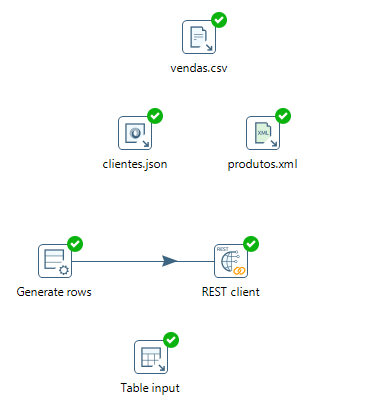
\includegraphics[width=0.7\textwidth]{imagens/e_extracao.png}
\caption{Fase E no Spoon -- extrações paralelas: CSV, JSON, XML, Generate+REST e Table Input.}
\label{fig:e_extracao}
\end{figure}

\begin{figure}[H]
\centering
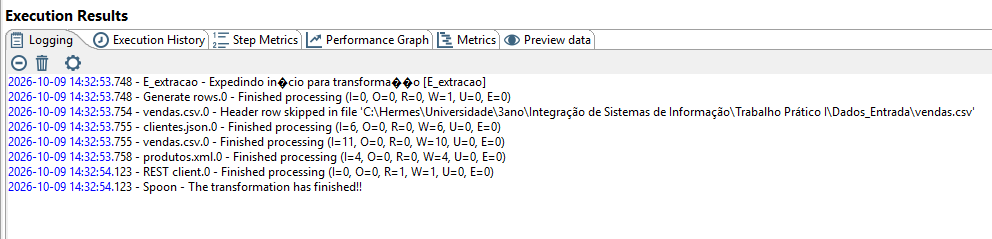
\includegraphics[width=0.9\textwidth]{imagens/e_log_rest_ok.png}
\caption{Registo de execução E\_extracao -- leitura das fontes e chamada REST.}
\label{fig:e_log}
\end{figure}

Os dados de entrada evidenciam os problemas a tratar: a Figura~\ref{fig:preview_sujo} mostra as 13 vendas com quantidade zero, duplicado V002, cliente nulo e data errada; a Figura~\ref{fig:preview_clientes} mostra os 6 clientes com correio inválido, correio nulo, NIF não numérico e duplicado; a Figura~\ref{fig:preview_produtos} mostra os 158 produtos com \textit{Loop XPath}; a Figura~\ref{fig:rest_preview} mostra a resposta 200 da API FakeStore obtida com \textit{trigger} Generate Rows; e a Figura~\ref{fig:preview_stock} mostra as 158 linhas de \textit{stock}.

\begin{figure}[H]
\centering
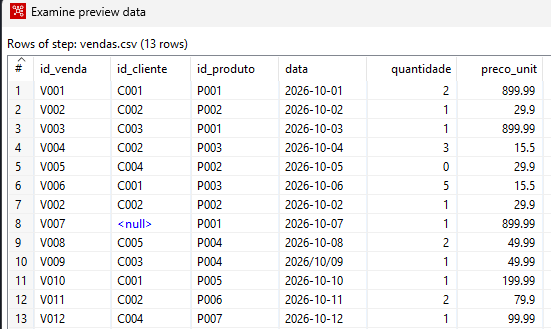
\includegraphics[width=0.9\textwidth,height=0.6\textheight,keepaspectratio]{imagens/preview_sujo.png}
\caption{Pré-visualização de vendas.csv -- 13 linhas com quantidade 0, duplicado V002, \texttt{id\_cliente} nulo e data errada.}
\label{fig:preview_sujo}
\end{figure}

\begin{figure}[H]
\centering
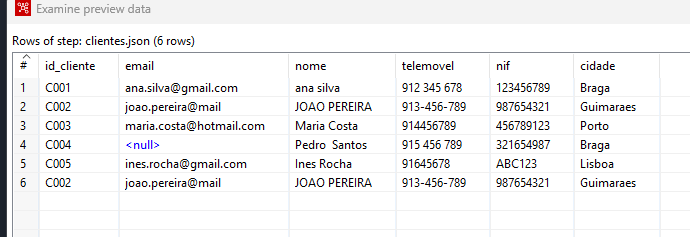
\includegraphics[width=0.9\textwidth,height=0.6\textheight,keepaspectratio]{imagens/preview_clientes.png}
\caption{Pré-visualização de clientes.json -- 6 linhas com correio inválido, \texttt{email} nulo, NIF ABC123 e duplicado.}
\label{fig:preview_clientes}
\end{figure}

\begin{figure}[H]
\centering
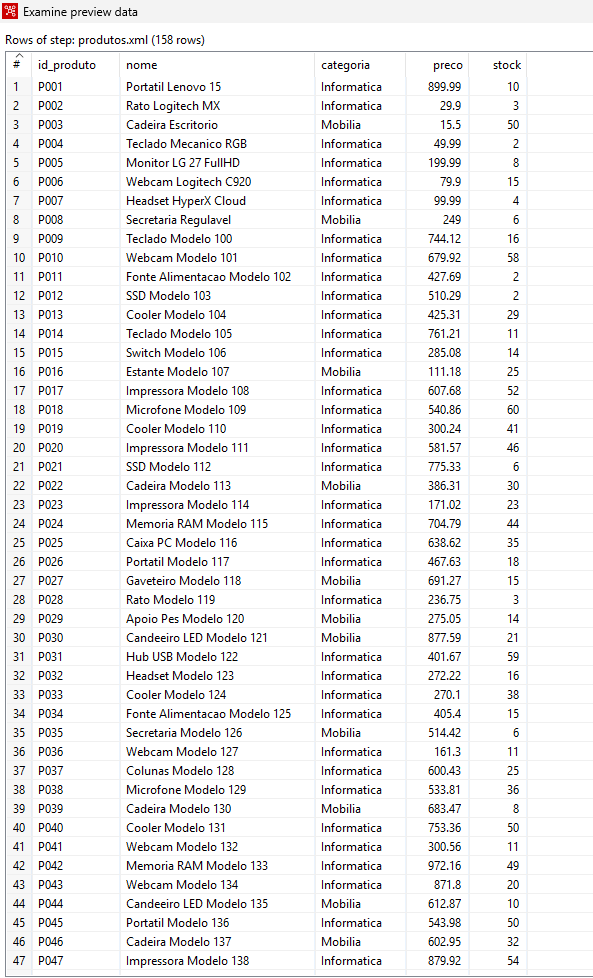
\includegraphics[width=0.85\textwidth,height=0.6\textheight,keepaspectratio]{imagens/preview_produtos.png}
\caption{Pré-visualização de produtos.xml -- 158 produtos (P001--P158) com \textit{Loop XPath} /produtos/produto.}
\label{fig:preview_produtos}
\end{figure}

\begin{figure}[H]
\centering
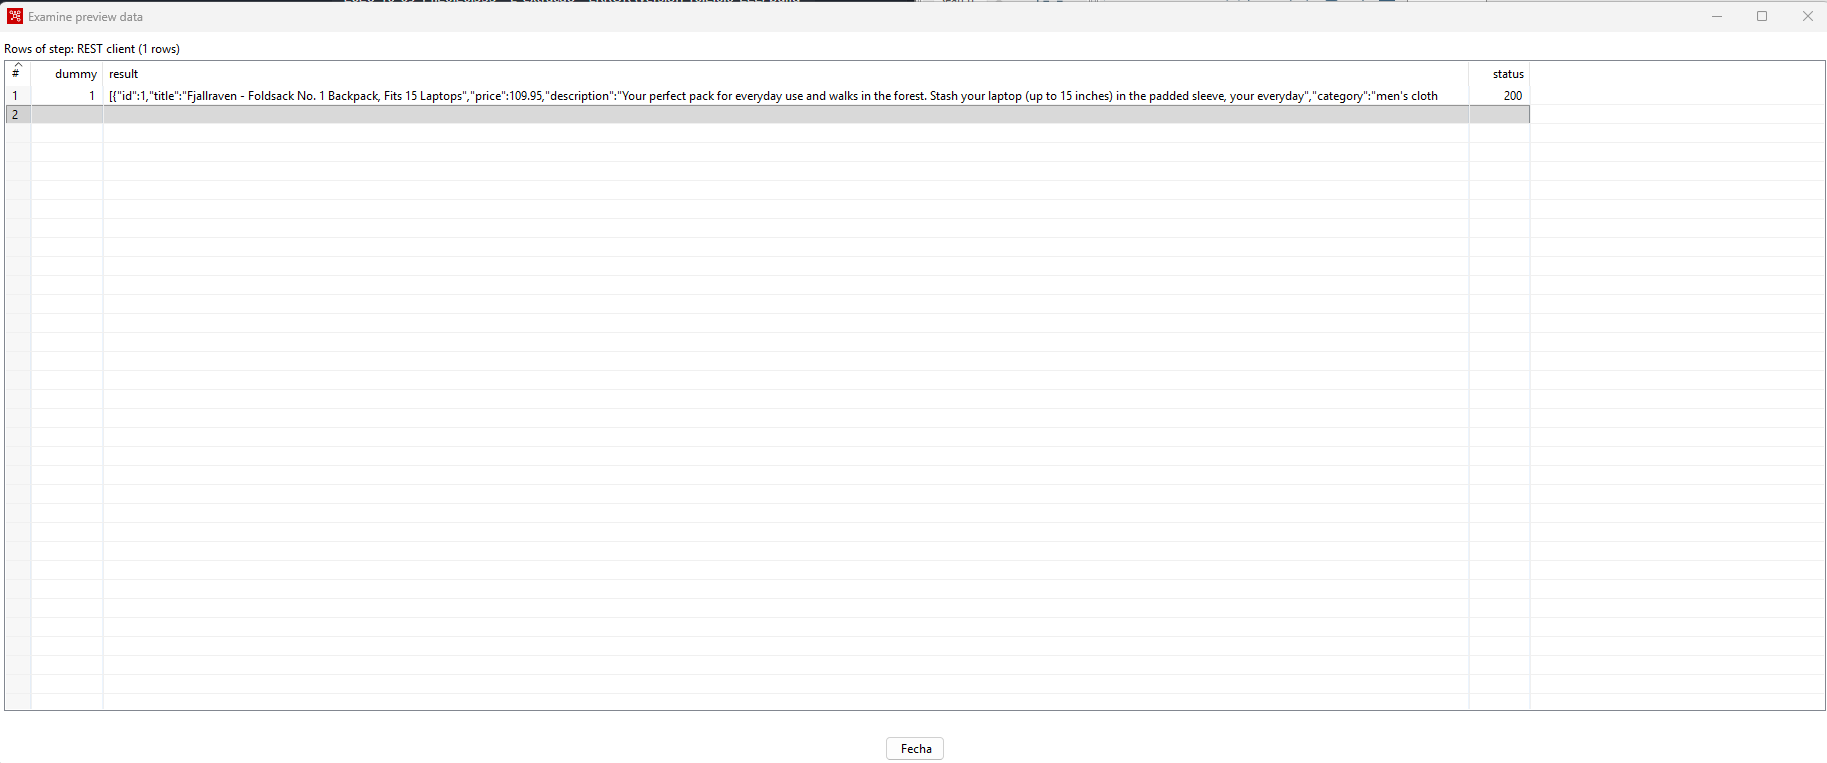
\includegraphics[width=0.85\textwidth]{imagens/rest_preview.png}
\caption{Pré-visualização do REST client -- 1 linha com estado 200 e JSON da FakeStore (\textit{trigger} Generate Rows dummy=1).}
\label{fig:rest_preview}
\end{figure}

\begin{figure}[H]
\centering
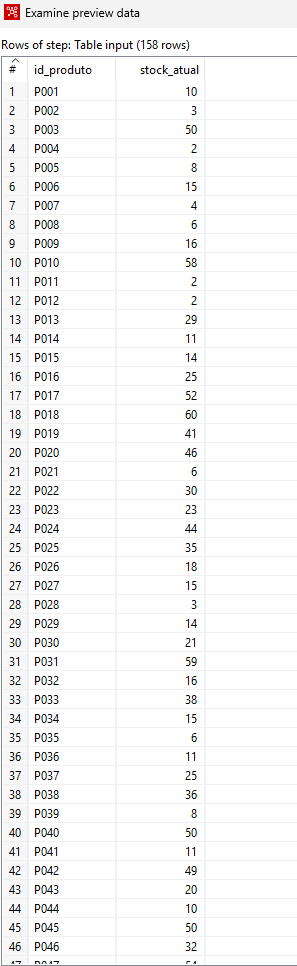
\includegraphics[width=0.55\textwidth,height=0.6\textheight,keepaspectratio]{imagens/preview_table_stock.png}
\caption{Pré-visualização do Table Input -- 158 linhas da tabela stock.}
\label{fig:preview_stock}
\end{figure}

\subsection{T\_limpeza.ktr}
Aplicou-se Sort Rows por \texttt{id\_venda} seguido de Unique Rows, que removeu o duplicado V002 (13 para 12), e Filter Rows com \texttt{quantidade\textgreater0 AND id\_cliente IS NOT NULL}, que removeu V005 e V007 (12 para 10), conforme a Figura~\ref{fig:filter10}. Efetuou-se a substituição da data de \texttt{/} para \texttt{-} (V009) e calculou-se \texttt{total\_linha=quantidade*preco\_unit} em Calculator BigNumber com precisão 2, após correção do \textit{locale} (Decimal \texttt{.} sem agrupamento), conforme a Figura~\ref{fig:preview_limpo}, com V001 a 1799.98.

\begin{figure}[H]
\centering
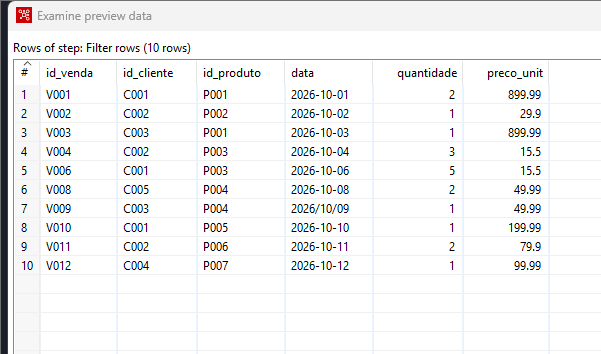
\includegraphics[width=0.9\textwidth,height=0.6\textheight,keepaspectratio]{imagens/filter_10.png}
\caption{Filter Rows vendas -- 10 linhas após remover quantidade 0 e id\_cliente null.}
\label{fig:filter10}
\end{figure}

\begin{figure}[H]
\centering
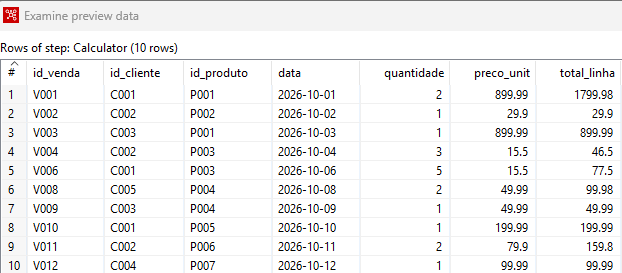
\includegraphics[width=0.9\textwidth,height=0.6\textheight,keepaspectratio]{imagens/preview_limpo.png}
\caption{Calculator final vendas -- 10 linhas com total\_linha correto (V001 1799.98).}
\label{fig:preview_limpo}
\end{figure}

\subsection{T\_clientes.ktr}
Normalizou-se o telemóvel com Replace por expressão regular \texttt{[\textbackslash s-]} (Figura~\ref{fig:replace_tel}), validaram-se correio eletrónico, telemóvel limpo e NIF em três avaliações Regex em série (Figura~\ref{fig:regex3}) e filtraram-se os triplos Y/Y/Y, restando 2 clientes limpos (C001 e C003), conforme a Figura~\ref{fig:clientes_limpos}. Aplicou-se anonimização para conformidade com o RGPD (Figura~\ref{fig:anon}).

\begin{figure}[H]
\centering
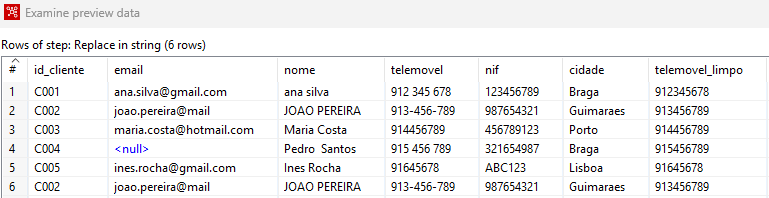
\includegraphics[width=0.95\textwidth]{imagens/replace_tel.png}
\caption{Substituição de telemóvel -- normalização com expressão regular [\textbackslash s-] (912 345 678 para 912345678).}
\label{fig:replace_tel}
\end{figure}

\begin{figure}[H]
\centering
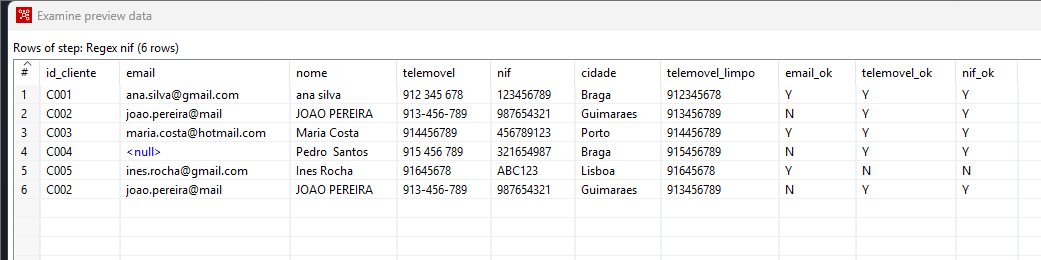
\includegraphics[width=0.95\textwidth]{imagens/regex_3.png}
\caption{Validação com expressões regulares -- 6 clientes com \texttt{email\_ok}, \texttt{telemovel\_ok} e \texttt{nif\_ok} (2 limpos C001/C003).}
\label{fig:regex3}
\end{figure}

\begin{figure}[H]
\centering
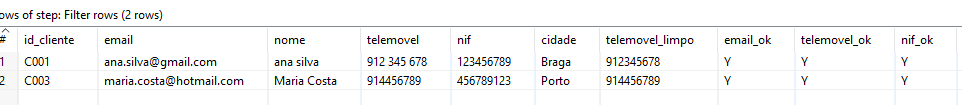
\includegraphics[width=0.9\textwidth]{imagens/clientes_limpos.png}
\caption{Clientes limpos -- 2 válidos após filtro Y/Y/Y com esquema remapeado.}
\label{fig:clientes_limpos}
\end{figure}

\begin{figure}[H]
\centering
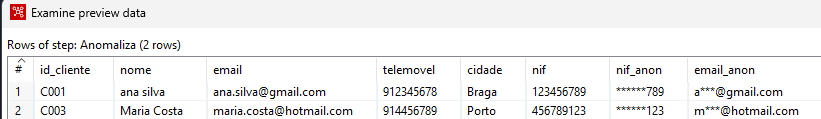
\includegraphics[width=0.9\textwidth]{imagens/anonimizacao.png}
\caption{Anonimização RGPD -- \texttt{nif\_anon} ******789 e \texttt{email\_anon} a***@gmail.}
\label{fig:anon}
\end{figure}

A Tabela~\ref{tab:regex} sistematiza as expressões regulares aplicadas na limpeza e validação dos dados.

\begin{table}[H]
\centering
\begin{tabular}{|l|l|}
\hline
Campo & Expressão regular \\ \hline
Correio eletrónico & \verb|^[A-Za-z0-9._%+-]+@[A-Za-z0-9.-]+\.[A-Za-z]{2,}$| \\ \hline
Telemóvel PT após limpar \verb|[\s-]| & \verb|^9[1236][0-9]{7}$| \\ \hline
NIF & \verb|^[0-9]{9}$| \\ \hline
Data & \verb|^\d{4}-\d{2}-\d{2}$| \\ \hline
\end{tabular}
\caption{Expressões regulares aplicadas.}
\label{tab:regex}
\end{table}

\subsection{T\_joins.ktr}
Efetuaram-se dois Stream Lookups, sem ordenação prévia, ao contrário do Merge Join: vendas com clientes por \texttt{id\_cliente} (Figura~\ref{fig:join1}) e o resultado com produtos por \texttt{id\_produto} (Figura~\ref{fig:joinfinal}). Os nulos em C002, C004 e C005 refletem integridade referencial, pois esses clientes foram filtrados como sujos. O diagrama completo encontra-se na Figura~\ref{fig:tjoin} e a agregação por cidade na Figura~\ref{fig:groupby}: sem cliente 436.17/5, Braga 2077.47/3 e Porto 949.98/2. Sem Sort prévio obtinham-se 9 linhas.

\begin{figure}[H]
\centering
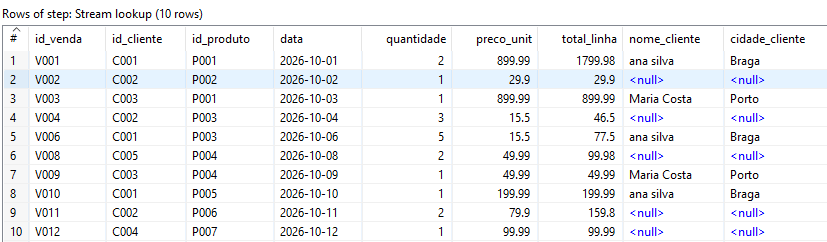
\includegraphics[width=0.9\textwidth,height=0.62\textheight,keepaspectratio]{imagens/join_clientes.png}
\caption{Junção 1 -- Stream Lookup vendas+clientes, 10 linhas, nulos por integridade referencial.}
\label{fig:join1}
\end{figure}

\begin{figure}[H]
\centering
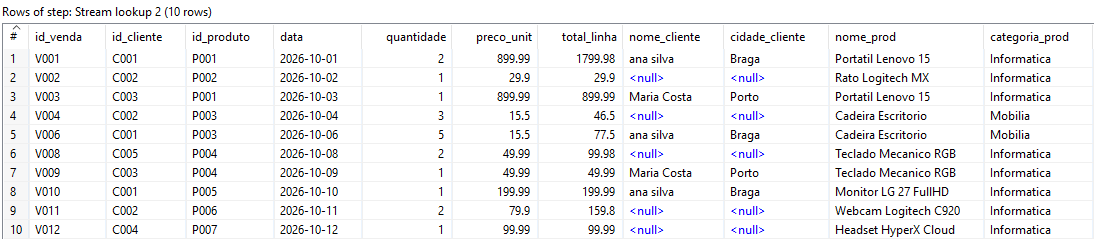
\includegraphics[width=0.9\textwidth,height=0.62\textheight,keepaspectratio]{imagens/join_final.png}
\caption{Junção final -- Stream Lookup 2 + produtos, 10 linhas com \texttt{nome\_prod} e \texttt{categoria\_prod}.}
\label{fig:joinfinal}
\end{figure}

\begin{figure}[H]
\centering
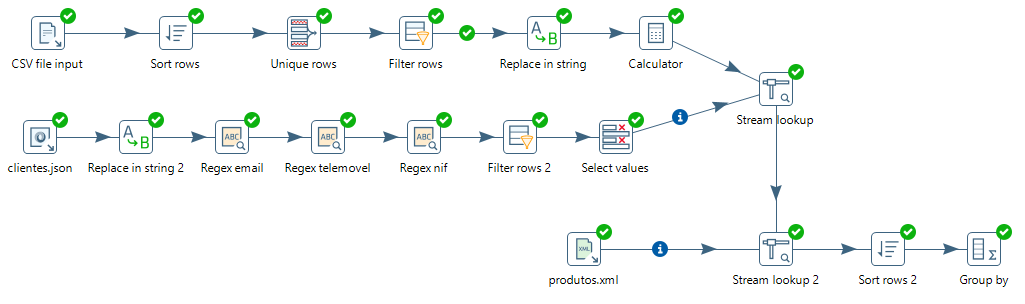
\includegraphics[width=0.8\textwidth]{imagens/t_join.png}
\caption{Diagrama T\_join completo -- vendas+clientes+produtos, 2 lookups, Sort+Group.}
\label{fig:tjoin}
\end{figure}

\begin{figure}[H]
\centering
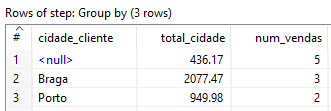
\includegraphics[width=0.6\textwidth]{imagens/groupby_3.png}
\caption{Group By \texttt{cidade\_cliente} -- 3 linhas: sem cliente 436.17/5, Braga 2077.47/3 e Porto 949.98/2.}
\label{fig:groupby}
\end{figure}

\subsection{L\_carga.ktr}
A transformação \texttt{L\_carga.ktr} materializa a fase de carga: persiste as vendas limpas em \texttt{dw\_vendas} e gera as exportações CSV e JSON. Antes da carga, confirmou-se a criação das tabelas e a ligação à base de dados. A Figura~\ref{fig:bd_tabelas} mostra as tabelas \texttt{dw\_vendas} e \texttt{stock}; a Figura~\ref{fig:bd_stock} o conteúdo de \textit{stock}; a Figura~\ref{fig:bd_dw} a tabela \texttt{dw\_vendas} vazia antes da carga; e a Figura~\ref{fig:db_ok} a ligação PostgreSQL testada com sucesso.

\begin{figure}[H]
\centering
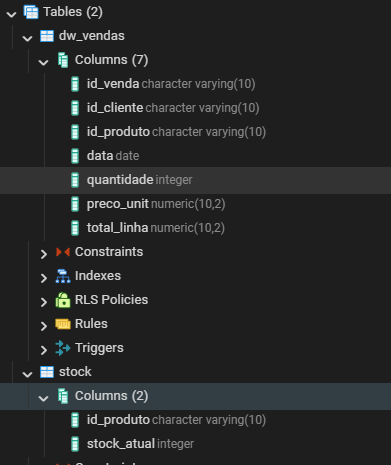
\includegraphics[width=0.6\textwidth]{imagens/bd_tabelas.png}
\caption{Tabelas \texttt{dw\_vendas} e \texttt{stock} na base de dados \texttt{isi\_store}.}
\label{fig:bd_tabelas}
\end{figure}

\begin{figure}[H]
\centering
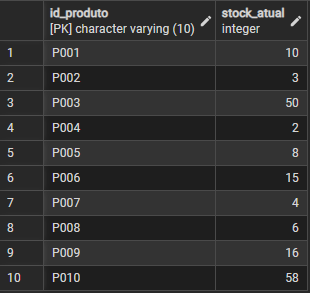
\includegraphics[width=0.8\textwidth]{imagens/bd_stock_conteudo.png}
\caption{Conteúdo da tabela \texttt{stock}.}
\label{fig:bd_stock}
\end{figure}

\begin{figure}[H]
\centering
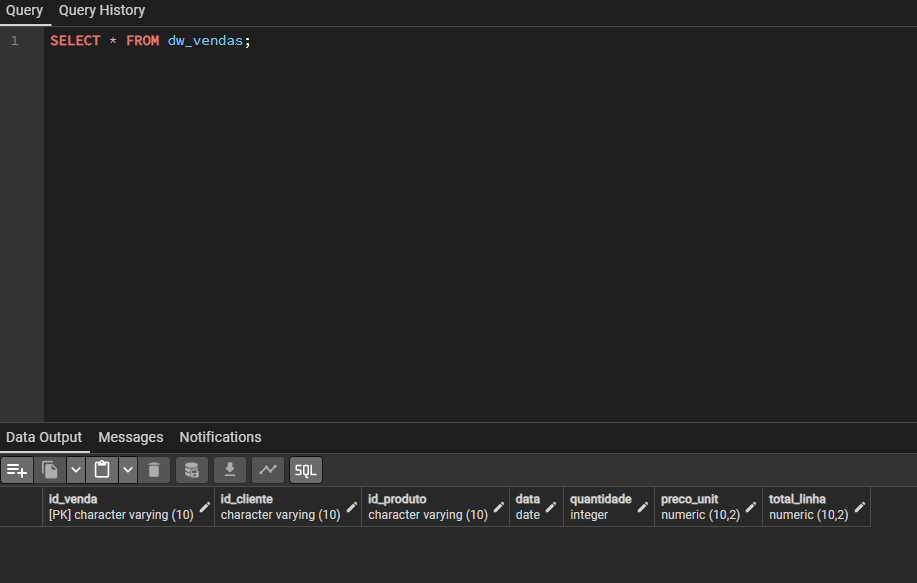
\includegraphics[width=0.8\textwidth]{imagens/bd_dw_vazia.png}
\caption{Tabela \texttt{dw\_vendas} vazia antes da carga.}
\label{fig:bd_dw}
\end{figure}

\begin{figure}[H]
\centering
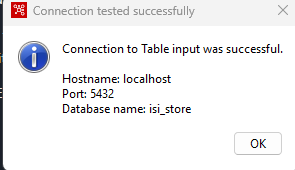
\includegraphics[width=0.6\textwidth]{imagens/db_connection_ok.png}
\caption{Ligação PostgreSQL \texttt{isi\_store} testada com sucesso.}
\label{fig:db_ok}
\end{figure}

A carga persistiu 10 linhas em \texttt{dw\_vendas} (Figura~\ref{fig:dwcheia}) e gerou \texttt{vendas\_limpas.csv}, com delimitador \texttt{;}, e \texttt{resumo.json} (Figura~\ref{fig:exports}), ambos transferidos para a pasta \texttt{data/output/ftp}, que simula o servidor remoto. A transformação de conversão gerou ainda \texttt{produtos.json} em \texttt{data/output}.

\begin{figure}[H]
\centering
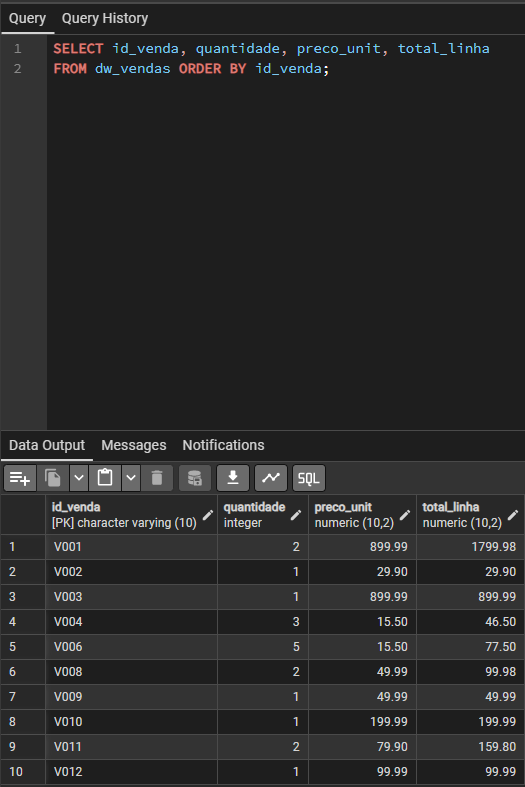
\includegraphics[width=0.85\textwidth,height=0.62\textheight,keepaspectratio]{imagens/dw_cheia.png}
\caption{Tabela \texttt{dw\_vendas} com 10 linhas e totais corretos (V001 1799.98).}
\label{fig:dwcheia}
\end{figure}

\begin{figure}[H]
\centering

\includegraphics[width=0.8\textwidth]{imagens/export_files.png}
\caption{Ficheiros exportados em \texttt{data/output}.}
\label{fig:exports}
\end{figure}

\subsection{T\_conversao.ktr}
A transformação de conversão reutiliza o catálogo de produtos e gera \texttt{produtos.json} com 158 registos no bloco \texttt{produtos}, preservando o preço com duas casas decimais. O diagrama encontra-se na Figura~\ref{fig:tconversao}.

\begin{figure}[H]
\centering
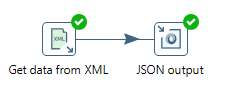
\includegraphics[width=0.8\textwidth]{imagens/t_conversao.png}
\caption{Conversão XML para JSON -- 158 produtos exportados para \texttt{produtos.json}.}
\label{fig:tconversao}
\end{figure}

% 5. Jobs
\section{Jobs}
O presente capítulo documenta o \textit{Job} principal, o painel complementar e a validação da execução. A Secção~5.1 apresenta o \textit{Job}; a Secção~5.2 o painel Node-RED; a Secção~5.3 a validação quantitativa; e a Secção~5.4 a discussão dos resultados.

\subsection{J\_principal.kjb}
Implementou-se o \textit{Job} com a sequência START, E\_extracao, T\_joins, L\_carga, T\_conversao, FTP\_csv, FTP\_json, Mail e Write to log, conforme a Figura~\ref{fig:job}, com execução integral válida. Utilizaram-se \textit{entries} Transformation para as quatro transformações, Send Mail para o alerta com os totais 2077.47, 949.98 e 436.17 (Figura~\ref{fig:mail}), FTP Put com um \textit{step} por ficheiro, devido à limitação da versão 10.2 a um \textit{wildcard} por \textit{step}, para o servidor local \texttt{127.0.0.1:21}, e Write to Log para registo de sucesso.

Importa distinguir as transformações de apoio \texttt{T\_limpeza} e \texttt{T\_clientes}, usadas para validar isoladamente as regras de limpeza, da transformação \texttt{L\_carga}, que integra a limpeza, a validação e as junções no fluxo orquestrado; o \textit{Job} executa E\_extracao, T\_joins, L\_carga e T\_conversao.

\begin{figure}[H]
\centering
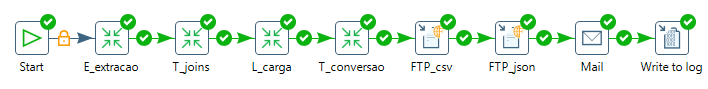
\includegraphics[width=0.95\textwidth]{imagens/job_ok.png}
\caption{\textit{Job} principal -- E, T, L, conversão, FTP CSV/JSON, Mail e Write to Log com sucesso.}
\label{fig:job}
\end{figure}

\begin{figure}[H]
\centering
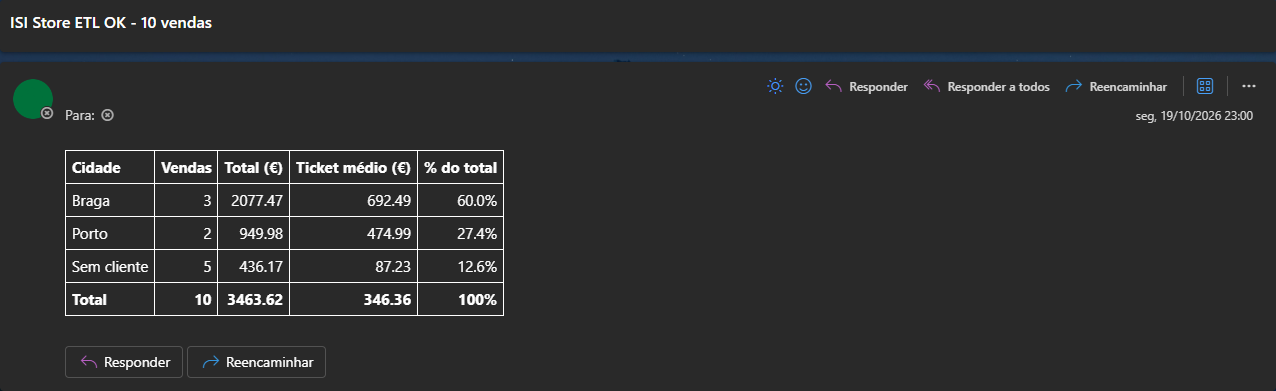
\includegraphics[width=0.8\textwidth]{imagens/email_ok.png}
\caption{Correio eletrónico de alerta com totais por cidade.}
\label{fig:mail}
\end{figure}

\subsection{Node-RED e painel}
Como ferramenta complementar, configurou-se o \textit{broker} Mosquitto em \texttt{localhost:1883}. O fluxo de \textit{streaming} republica em ciclo as vendas reais de \texttt{vendas\_limpas.csv} no tópico \texttt{isi/vendas} (Figura~\ref{fig:nrflow}), e o painel lê o mesmo CSV para calcular indicadores ETL, receita e ticket médio por cidade, principais produtos, tabela por cidade e tabela de vendas em \textit{streaming} MQTT (Figura~\ref{fig:nrdash}), disponível em \url{http://localhost:1880/ui}.

\begin{figure}[H]
\centering
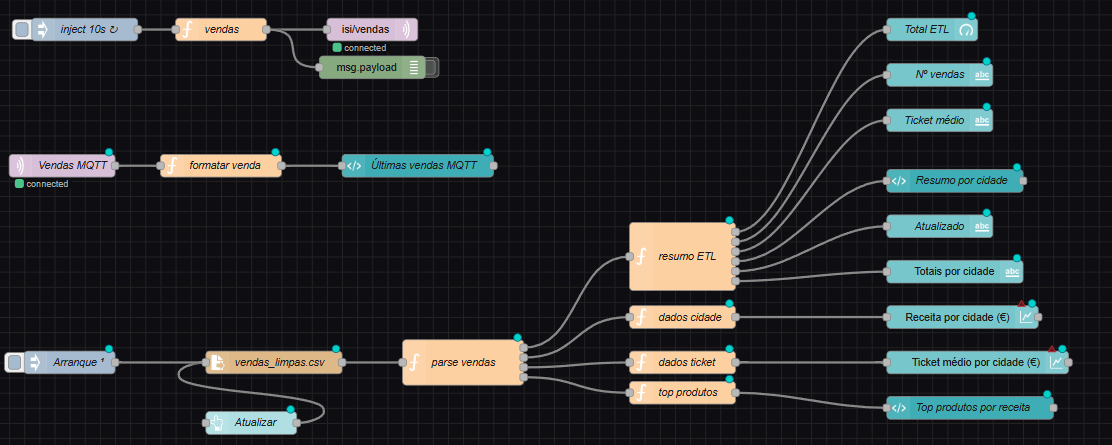
\includegraphics[width=0.9\textwidth]{imagens/nodered_flow.png}
\caption{Fluxos Node-RED -- \textit{streaming} isi/vendas, agregação e painel.}
\label{fig:nrflow}
\end{figure}

\begin{figure}[H]
\centering
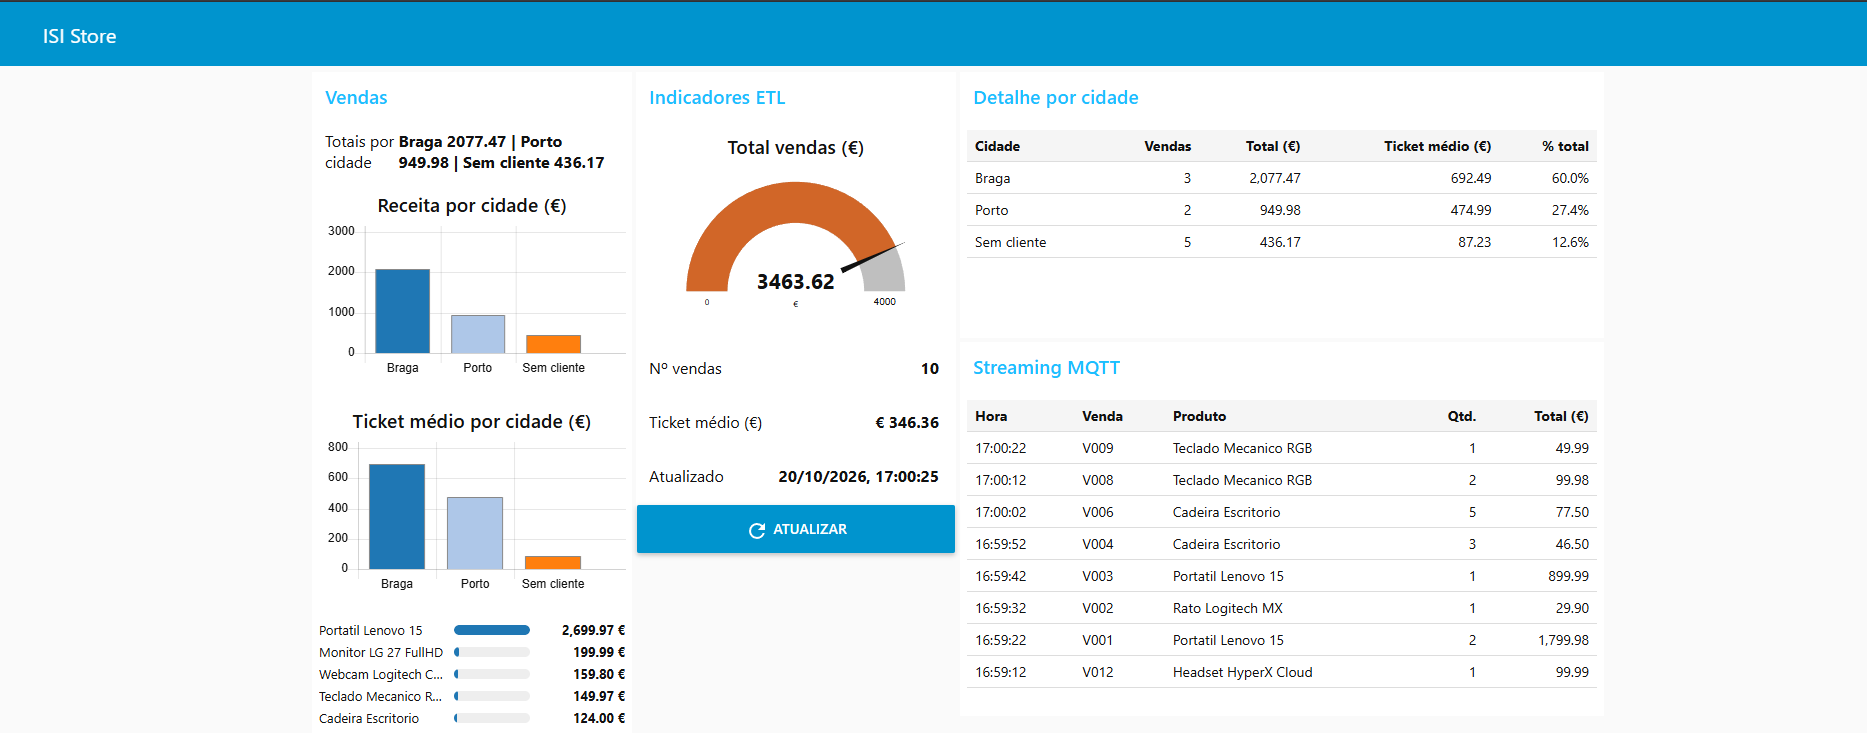
\includegraphics[width=0.9\textwidth]{imagens/nodered_dashboard.png}
\caption{Painel calculado a partir de \texttt{vendas\_limpas.csv}: indicadores ETL (total 3463.62), receita e ticket médio por cidade, principais produtos, tabela por cidade e \textit{streaming} MQTT.}
\label{fig:nrdash}
\end{figure}

\subsection{Validação da execução}
A Tabela~\ref{tab:resultados} sintetiza as contagens obtidas e as evidências associadas. A execução integral do \textit{Job} terminou com sucesso e produziu os ficheiros e os registos esperados.

\begin{table}[H]
\centering
\small
\begin{tabular}{|p{2.6cm}|p{4.0cm}|p{3.4cm}|p{3.0cm}|}
\hline
Etapa & Entrada & Saída & Evidência \\ \hline
Extração & 13 vendas, 6 clientes, 158 produtos, 1 REST e 158 \textit{stock} & 5 fontes lidas & Figura~\ref{fig:e_log} \\ \hline
Limpeza de vendas & 13 linhas & 10 linhas & Figura~\ref{fig:filter10} \\ \hline
Validação de clientes & 6 registos & 2 válidos & Figura~\ref{fig:clientes_limpos} \\ \hline
Junção e agregação & 10 vendas & 3 grupos por cidade & Figura~\ref{fig:groupby} \\ \hline
Carga & 10 vendas & 10 linhas em \texttt{dw\_vendas} & Figura~\ref{fig:dwcheia} \\ \hline
Exportação & 10 vendas & CSV e JSON & Figura~\ref{fig:exports} \\ \hline
Conversão & 158 produtos & \texttt{produtos.json} & Figura~\ref{fig:tconversao} \\ \hline
Orquestração & \textit{Job} completo & Sucesso, correio e FTP & Figuras~\ref{fig:job} e \ref{fig:mail} \\ \hline
\end{tabular}
\caption{Síntese das contagens e evidências da execução.}
\label{tab:resultados}
\end{table}

A Tabela~\ref{tab:resultados} confirma que o processo cumpriu as três fases obrigatórias: extração multiformato, transformação com limpeza e agregação, e carga com orquestração. Os totais por cidade foram Braga 2077.47/3, Porto 949.98/2 e sem cliente 436.17/5, num total de 3463.62 e ticket médio de 346.36.

\subsection{Discussão dos resultados}
A discussão organiza-se em três dimensões: qualidade e integridade dos dados, integração e orquestração, e limitações do trabalho.

\subsubsection{Qualidade e integridade dos dados}
A limpeza reduziu 13 vendas a 10. O duplicado V002 foi eliminado por Sort Rows e Unique Rows; V005 foi rejeitada por quantidade zero; V007 foi rejeitada por cliente nulo; e V009 foi corrigida pela substituição de \texttt{/} por \texttt{-}. A validação de clientes reduziu 6 registos a 2, após verificação de correio eletrónico, telemóvel e NIF.

A existência de vendas sem cliente deve ser interpretada como consequência da integridade referencial: os clientes inválidos foram excluídos, mas as vendas associadas permaneceram para não perder receita. O grupo sem cliente, com 436.17 e 5 vendas, evidencia a importância de distinguir dados ausentes de dados inválidos e de documentar essa decisão.

\subsubsection{Integração e orquestração}
O \textit{Job} encadeou as transformações e as tarefas complementares sem intervenção manual. O correio eletrónico comunicou os totais por cidade, o FTP transferiu os ficheiros e o \textit{log} registou o sucesso. Esta orquestração reduz o esforço operacional e torna a execução repetível.

O painel Node-RED complementa a integração \textit{batch} com uma leitura do CSV consolidado e uma tabela de \textit{streaming} MQTT. A atualização periódica permite observar vendas recentes, mas não substitui a fonte de verdade: o painel depende do ficheiro produzido pelo ETL.

\subsubsection{Limitações e ameaças à validade}
O FTP foi configurado num servidor local, devido à ausência de DNS externo no laboratório, pelo que a transferência não representa um ambiente de produção. Os dados são sintéticos e a execução foi validada numa única execução integral, o que limita a generalização dos resultados.

O painel não tem autenticação nem controlo de acessos. Além disso, a dependência de \texttt{vendas\_limpas.csv} introduz uma etapa manual entre o ETL e a atualização dos indicadores. O ficheiro \texttt{produtos.json} foi gerado localmente e não foi incluído na transferência FTP. Estas limitações não invalidam o processo, mas delimitam o seu âmbito.

% 6. Vídeo com demonstração
\section{Vídeo com demonstração (QR Code)}
O vídeo tem 2 minutos e demonstra a execução do \textit{Job}, os dados de entrada sujos, os resultados limpos, o correio eletrónico e o painel.
\begin{center}

\includegraphics[width=5cm]{imagens/qrcode.png}\\
\small QR code para o vídeo de demonstração.
\end{center}

% 7. Conclusão e Trabalhos futuros
\section{Conclusão e Trabalhos futuros}
O presente capítulo sintetiza o trabalho, identifica as contribuições, reconhece as limitações e propõe trabalhos futuros. A Secção~7.1 apresenta a síntese e as contribuições; a Secção~7.2 as limitações; e a Secção~7.3 os trabalhos futuros.

\subsection{Síntese e contribuições}
O trabalho cumpriu as três fases obrigatórias do enunciado: extração multiformato validada por contagens, transformação com limpeza, expressões regulares, anonimização, junções e agregação, e carga com orquestração completa, incluindo correio eletrónico, FTP e registos. A execução produziu 10 vendas limpas, 2 clientes válidos, 158 produtos integrados e 10 linhas no \textit{Data Mart}.

As contribuições principais são: (i) um processo ETL reprodutível para a ISI Store; (ii) uma especificação de requisitos e uma arquitetura lógica; (iii) regras de qualidade e anonimização alinhadas com o RGPD; (iv) a integração de orquestração, notificação e visualização; e (v) documentação que permite repetir e avaliar o processo. A comparação de plataformas e a discussão dos resultados constituem a componente de investigação aplicada.

\subsection{Limitações}
As limitações incluem o FTP local, a natureza sintética dos dados, a dependência do painel em relação ao CSV, a ausência de autenticação no painel e a inexistência de um agendador de produção. A validação numa única execução integral também limita a avaliação de desempenho e de robustez.

\subsection{Trabalhos futuros}
Como trabalhos futuros propõem-se a persistência em MongoDB, a visualização em Grafana em tempo real, a orquestração com Apache Airflow, a inclusão de testes automáticos de qualidade, a autenticação do painel e a integração do \texttt{produtos.json} no fluxo FTP. Propõe-se ainda a comparação com uma arquitetura de \textit{streaming} baseada em Kafka ou MQTT industrial.

% 8. Referências Web
\section{Referências Web}
\begin{itemize}
\item Ferreira, L. e Ribeiro, Ó. (2026). \textit{Enunciado do Trabalho Prático I de ISI}. IPCA.
\item Hitachi Vantara (2026). \textit{Pentaho Data Integration Documentation}. \url{https://www.hitachivantara.com/}
\item Node-RED (2026). \url{https://nodered.org/}
\item Eclipse Mosquitto (2026). \url{https://mosquitto.org/}
\item PostgreSQL (2026). \url{https://www.postgresql.org/}
\item FakeStore API (2026). \url{https://fakestoreapi.com/}
\end{itemize}

\appendix
\section{Contagens de validação}
Registaram-se as seguintes contagens ao longo do processo: \texttt{vendas.csv} com 13 linhas, \texttt{clientes.json} com 6 objetos, \texttt{produtos.xml} com 158 produtos, tabela \texttt{stock} com 158 linhas, vendas limpas com 10 linhas, clientes válidos com 2 registos, \texttt{dw\_vendas} com 10 linhas e Group By com 3 linhas.

\end{document}
